\chapterimage{advice.pdf}
\chapterimagecaption{\textit{The Thinker} (1904) by Auguste Rodin}

\chapter{Program Advice}

\section{Graduate Program}

The Physics Department at McGill offers excellent research in a broad range of fields. Graduate studies are offered at the Masters and PhD level. Graduate students will be embedded in one of the department's research groups and work on a specific topic under the guidance of their supervisor.

    \subsection{MSc Requirements} \index{MSc Requirements}

    Complete details of degree requirements can be found \href{https://www.physics.mcgill.ca/grads/requirements.html}{here}.

    \subsubsection{Courses}

    Official course recommendations can be found \href{https://www.physics.mcgill.ca/grads/courses.html}{here}. Note that the department lists recommended courses according to your area of study. You do NOT \textit{need} to follow this recommendation, as long as you and your supervisor agree on which courses you should take based on your interest/research. You are also more than welcome to take courses outside the department/university, see the next section for more information.

    Students need to do 5 courses worth 3 credits each, and at least one of the 5 must be at the 600 level or higher. A minimum of 2 of these 5 courses must be a PHYS course at McGill. The other 3 courses may be either physics or non-physics courses, and a maximum of 2 of those 3 courses may be taken outside McGill. If you take 2 or more courses at McGill at the 600 or 700 level, you may request to use one of them as an exemption for your PhD. Students also need to register for professional development courses PHYS 601/PHYS 602 in their first year. 

    \begin{plainexercise}
            \textbf{DO NOT FORGET}: Register for research courses PHYS 693 (3) in your first year and thesis course PHYS 690 (12 + 12 credits) in your second year. 
    \end{plainexercise}

    \subsubsection{Thesis} \index{Thesis}

    All details for writing/submitting a thesis can be found \href{https://www.mcgill.ca/gps/thesis}{here}. There are specific deadlines that you need to submit your thesis draft by to ensure your status is "Thesis Evaluation" which entitles you to a much lower tuition during the next semester if you plan on being enrolled in the same program for another semester. GPS provides the table below listing all the deadlines and graduation dates.

    \begin{figure}[hbt]
        \centering
        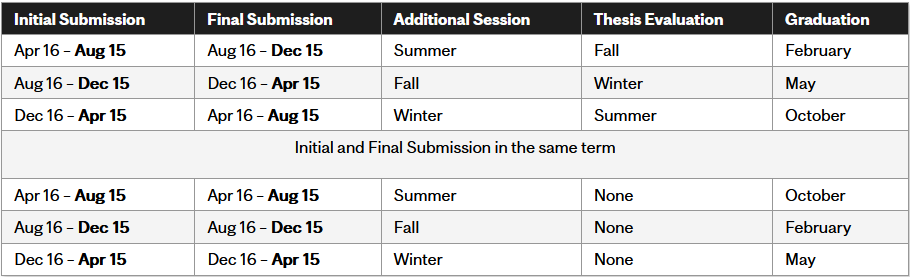
\includegraphics[width=0.9\linewidth]{Pictures/thesis_submission_deadlines.png}
        \label{fig:thesis_submission_deadlines}
    \end{figure}


    \begin{plaincorollary}
        The term after you submit your initial thesis is referred to as your thesis evaluation term which reduces the amount of tuition that you have to pay. For example: if you submit your thesis at the end of April, the summer term will count as your thesis evaluation term. You would need to make your final submission before the end of August if you wish to graduate in October.
    \end{plaincorollary}

    \subsection*{MSc Timeline}
    Here's a sample timeline for students starting their MSc program in Fall. You need not follow this exact roadmap. Use \href{https://horizon.mcgill.ca/myprogress/ResponsiveDashboard/}{myProgress} for a more comprehensive timeline and refer to \href{https://www.physics.mcgill.ca/grads/courses.html}{this} website for complete coursework requirements. The course credits are mentioned in the parenthesis.

    \begin{vtimeline}[description={text width=12cm}, row sep=2ex]
        Sem 1 & PHYS 601 (3) + PHYS 693 (3) + 2 Courses (3+3) \endlr 
        Sem 2 & PHYS 602 (3) + 2 Courses (3+3)\endlr
        Sem 3 & PHYS 690D1 (12) + 1 Course (3) \endlr
        Sem 4 & PHYS 690D2 (12) + Initial Thesis Submission\endlr
        Summer & Final Thesis Submission \endlr
    \end{vtimeline}

    If you join the program in the winter, you can do PHYS 602 in your first semester and then PHYS 601 in your second. These two courses can be taken in any order but they must be taken in consecutive terms. The research courses 690 and 693 remain in progress on your transcript untill you are granted a degree by the senate.
    
    It is recommended to take as many complementary courses in your first year so that you have more available time to focus on your thesis in your second year.

    \subsection{Fast-Tracking} \index{Fast-Tracking}
        On the recommendation of the Departmental Graduate Committee, fast-tracking from the M.Sc. program into the Ph.D. program may be granted after one year, if:  the student has fulfilled the M.Sc. coursework requirements, or;
        the candidate's Supervisor determines that the student qualifies based on the student's academic and research record.

        It is recommended to talk to your supervisor about fast-tracking! It has pros and cons, so please chat with your peers/supervisor to see if this is the best option for you.

        \textbf{If you do end up fast-tracking}, you will be a ``\textbf{PhD1}'' in your first year, which means that you will \textit{need} to register for the following courses: PHYS 715 PhD1 Research Credit Course 1 and PHYS 716 PhD1 Research Credit Course 2. These will be taken consecutively in your first year. 
    
    \subsection{PhD Requirements} \index{PhD Requirements}

    Complete details of degree requirements can be found \href{https://www.physics.mcgill.ca/grads/requirements.html}{here}. Candidates starting their PhD directly from a Bachelor's degree in Physics are referred to as ``\textbf{PhD1}''. Candidates entering their PhD program with an MSc degree in Physics or equivalent qualification are referred to as ``\textbf{PhD2}''.

     PhD1 students are required to take 30 research credits (PHYS 715 and PHYS 716) upon entry to the program. And they must complete 6 3-credit graduate courses at the 500 or 600 level or above, with at least three being at the 600 level. 
     
     PhD2 students need to do 2 3-credit graduate courses at the 600 level or above. One of the courses can be substituted if the student completed his MSc at McGill. 
    
    \subsubsection{Courses}
    
    Official course recommendations can be found \href{https://www.physics.mcgill.ca/grads/courses.html}{here}. Note that the department lists recommended courses according to your area of study. You do NOT \textit{need} to follow this recommendation, as long as you and your supervisor agree on which courses you should take based on your interest/research. You are also more than welcome to take courses outside the department/university, see the next section for more information. Students who did their undergrad at McGill may transfer 1 course for graduate credit if they did not need it to complete their undergraduate degree.

    \subsubsection{Letter of Understanding} \index{Letter of Understanding}

    The letter of understanding (LOU) is a way for you and your supervisor to be on the same page in terms of your research objectives, goals, and timeline. This is meant to be structured as a conversation and helps with communication and transparency. 

    Details on the generating this letter of understanding can be found \href{https://www.physics.mcgill.ca/grads/lou22.pdf}{here}.

    \subsubsection{Supervisory Committee}

    Your supervisory committee is a group of 3 professors (including your supervisor) meant to serve as your guides throughout the course of your PhD (think of it as an Order of Jedi to your young Padawan self). A meeting with your supervisory committee will be a yearly checkpoint to see how your research is progressing.

    For these checkpoints, you need to fill out the \href{https://www.mcgill.ca/gps/students/progress-tracking}{Graduate Student Progress Tracking Form} and submit it to GPS. 
    
    \subsubsection{Prelim} \index{Prelim}

    The prelim should be taken within 2.5 years of your program start date for PhD 1 students and within 1.5 years for PhD 2 students. This exam is aimed at testing undergraduate physics knowledge related to your research project, along with your understanding of your research problem and subfield. It has two components:
    \begin{itemize}
        \item A 10-page research proposal 
        \item An oral exam, which includes a 20 minute presentation and a 1-1.5hr question period.
    \end{itemize}

    The prelim committee consists of 4 people: your supervisory committee plus one prelim chair (a professor from a different research area).

    A lot more information about prelims (and in much more detail) can be found \href{https://www.physics.mcgill.ca/grads/prelim-candidate.html}{here}.

    In case of failure on your first try, you are allowed one final second attempt.

    Students who have taken the prelim in the past few years recommend confirming your prelim committee at least 2.5 months before the date of the exam. Usually, the availability of professors acts as the biggest obstacle. Since December is usually a busy time, if you can, try scheduling your prelim for end of November (this is not compulsory, just a suggestion; a lot of people still do prelims in December). It is also worth asking your supervisor which professors might be the best fit for your committee. 
    
    Although generally advertised as testing undergraduate knowledge, the latter part of the oral exam may involve questions about your research and your knowledge of the field. Expect to be challenged with hard questions -- most people find it to be so and it is not a reflection of how your exam is going. Professors may progressively ask harder questions to help you structure the direction of your research.

    \subsubsection{Thesis} \index{Thesis}

    All details for writing/submitting a thesis can be found \href{https://www.mcgill.ca/gps/thesis}{here}. 

    \subsection*{PhD Timeline}
    Here's a sample timeline for students starting at the PhD2 level in Fall. You need not follow this exact roadmap. Use \href{https://horizon.mcgill.ca/myprogress/ResponsiveDashboard/}{myProgress} for a more comprehensive timeline and refer to \href{https://www.physics.mcgill.ca/grads/courses.html}{this} website for complete coursework requirements. The course credits are mentioned in the parenthesis.

    \begin{vtimeline}[description={text width=14cm}, row sep=2ex]
        Sem 1 & PHYS 601 (3) + PhD2 Progress Tracking + 1 or 2 Courses (3+3) + LOU \endlr 
        Sem 2 & PHYS 602 (3) \endlr
        Summer & Prelim Prep (Report) \endlr
        Sem 3 & PHYS 700 (Prelim) =  PhD3 Progress Tracking \endlr
        Sem 4 &  \endlr
        Sem 5 &  PhD4 Progress Tracking \endlr
        Sem 6 & Individual Development Plan (IDP)  \endlr
        Sem 7 & PhD5 Progress Tracking\endlr
        Sem 8 & Initial Thesis Submission \endlr
        Summer & Final Thesis Submission \endlr
    \end{vtimeline}

    \section{Taking courses in a different department/university}\index{Courses outside McGill}
        It is entirely possible to take a course in a different department/university and still get credited for your degree. Note that although the physics department website outlines the courses that you \textit{should} be taking, it is entirely up to you and your supervisor to decide which courses will most benefit you and your research. This section will focus on the different ways in which you can take a course outside of the McGill physics department. 

        \subsection{Courses outside the Department Area}

        Depending on your research area, it might be wise to take a course outside of the physics department, such as, but not limited to, in the chemistry, engineering, and biology departments.

        Some supervisors encourage students to think as broadly as possible when planning their courses, which may involve taking more than the two out-of-department courses technically allowed for MSc and direct-entry PhD students. As long as the courses are relevant to your research area and you justify this to the GPC, this rule is quite flexible in practice. 

        \subsection{Courses outside the University}

There will be opportunities, often sent via email, to take courses at a different university. Many universities also offer courses to students in different institutions without publicising them. If you find that McGill does not offer enough relevant courses to fulfil program requirements, you might want to check the other universities in Québec or even Canada.

\subsubsection{Québec Universities}

The process for Québec universities is pretty simple, and McGill has a \href{https://www.mcgill.ca/transfercredit/iut}{page specifically for it}:
\begin{enumerate}
    \item Go on the \href{https://aehe.bci-qc.ca/en}{AEHE portal}.
    \item Click on "Applications" and select McGill as your home institution.
    \item Log in with your McGill student account.
    \item Accept the terms of use and click "Submit".
    \item Accept the information transfer description. Change the frequency of verification if desired.
    \item Select "Student" as your occupation.
    \item Agree to the terms and conditions again.
    \item Click on "New Application"
    \item Log in with your McGill credentials (if not automatically redirected to the log-in window, click on Azure SSO)
    \item Verify that the information provided is correct
    \item Select the correct program is not already selected
    \item Select the appropriate semester and click on "Create Request"
    \item Add your desired class by looking up the host university and location
    \item Add the desired class by double-clicking it and filling out the information. 
    \begin{itemize}
        \item The schedule and section are only truly relevant when the same class is offered in multiple instances, but you should fill it out nonetheless
        \item Try to find the closest equivalent at McGill to add in the replacement section
        \item In the comments, briefly describe why you are taking a class outside McGill
    \end{itemize} 
    \item Once you have added the desired course, you can submit the application.
\end{enumerate}
It might take a while to hear back from the host university. It is recommended that you stay in contact with the prof directly so that you can be updated on the course start date and the first few assignments and documents in case you do not have access to the host university's website in time. 

\subsubsection{Other Canadian Universities}
The exact process varies across universities. General advice from people who took a class at another university: contact the graduate coordinator for the physics program at the host university directly. They will send you the relevant forms. This should be done as soon as possible as the process can be long and arduous. 

In addition, for courses outside McGill (both in Québec and outside Québec), the course grades cannot be transferred. This means that these course grades will be pass/fail (or Satisfactory/Unsatisfactory in McGill terminology) and you will only get the credit but it will not count towards your GPA. Students must also make sure that the courses are offered by an institution in some sort of graduate exchange agreement (e.g. these is one between McGill, UBC, UdeM, and UToronto). Through these exchange agreements, students do not pay tuition to the school at which they are taking a course. Students must provide official syllabi for the courses (which cannot be a PDF of the course website according to the Faculty of Sciences) and then pay to officially send the transcript from said school to McGill after the term ends. 


     
        